% Chapter Template

\chapter{Introducció i estat de l'art} % Main chapter title

\label{Context} % Change X to a consecutive number; for referencing this chapter elsewhere, use \ref{ChapterX}

Aquest projecte és un Treball Final de Grau de l'especialitat d'Enginyeria del Software de la Facultat d'Informàtica de Barcelona (Universitat Politècnica de Catalunya). Es tracta d'un projecte de modalitat A que pretén crear una aplicació de suport al viatger.

%----------------------------------------------------------------------------------------

\section{Formulació del problema}

Viatjar ajuda a veure la vida des de perspectives diverses, aquest és un dels motius pels quals cada dia tothom està més disposat a emprendre viatges arreu del món. Existeixen molts perfils diferents de viatgers, a alguns els agrada descobrir natura, a d’altres les grans ciutats, hi ha qui es decanta per la tranquilitat i qui prefereix l’aventura. Sigui quin sigui l’enfoc del viatge, el propòsit és aprendre alguna cosa que quedi per al record.\\

En els darrers anys, com a conseqüència d’internet i l’abaratiment de les companyies low cost, és molt més fàcil desplaçar-se i estar informat sobre els diferents racons del món. És important també tenir en compte que la gran majoria de gent disposa d’un smartphone, aquest fet permet al viatger accedir a internet durant el viatge i, per tant, estar connectat constantment, cosa que simplifica molt l’accés a informació al moment.\\

Les persones ens adaptem molt ràpidament a les coses que ens són més fàcils de fer, per aquest motiu actualment no es planifica tant i sovint es necessita una eina que permeti solucionar un problema a l’instant. És en aquest context on apareix l’aplicació que pretén desenvolupar aquest projecte.\\

Durant un viatge sorgeixen moltes necessitats com poden ser: buscar un restaurant, informar-se del temps, buscar transport, portar un control de les despeses, etc. Actualment existeixen varies aplicacions que ataquen parts concretes d’aquest problema però això obliga al viatger a tenir moltes aplicacions instal·lades al seu dispositiu sense comunicació entre elles.\\

La idea que proposa aquest projecte és construir una aplicació que englobi les funcionalitats que un viatger considera més importants durant el transcurs del seu viatge presentant-li la informació filtrada tenint en compte el seu estil de viatjar. D’aquesta manera podem definir els objectius del projecte.\\

Aquest projecte té quatre objectius molt clars:
\begin{itemize}
\item{\textbf{Donar suport al viatger durant el transcurs del seu viatge:}} el viatger necessita suport de diversos tipus durant el viatge, per aquest motiu, s’han dut a terme entrevistes a viatgers que han servit per orientar i definir les funcionalitats que vol oferir l’aplicació. Aquestes són: gestió econòmica, previsió metereològica, gestió de cerques de llocs d’interès, gestió d’emergències, cerca de transports, cerca d’imatges i gestió de notes.\\

\item{\textbf{Ser intermediari en l’ús de diverses aplicacions que ajuden al viatger:}} actualment existeixen diverses aplicacions especialitzades en les funcionalitats que aquesta vol implementar. L’objectiu es basa en utilitzar algunes de les aplicacions disponibles en el mercat per tal de crear funcionalitats pròpies i d’aquesta manera obtenir una aplicació completa per al suport al viatger. 

\item{\textbf{Personalitzar les dades obtingudes per a cada viatger:}} qualsevol persona pot emprendre un viatge, per tant, els viatgers no tenen unes preferències establertes, hi ha molta diversitat d’estils. Per aquest motiu aquesta aplicació planteja la personalització dels viatges per tal de filtrar la informació obtinguda a través de l’accés a d’altres aplicacions i així ser capaç d’oferir a l’usuari el que s’ajusta més al seu estil.

\item{\textbf{Ser fàcilment escalable:}} el món de la tecnologia és un món canviant, per aquest motiu aquesta aplicació vol estar preparada per agregar o eliminar funcionalitats de la manera més senzilla possible.

\end{itemize}

\section{Parts interessades}

Aquest projecte va adreçat a satisfer les necessitats d’un sector molt ampli de població, no estem parlant d’un client concret. Les parts interessades poden tenir objectius molt diversos. En aquest projecte definim les següents parts interessades:
\begin{itemize}

\item\textbf{Viatgers}\\
Els viatgers són els principals protagonistes, són els que es beneficien de l’aplicació de forma directa.

\item\textbf{Ajuntaments}\\
Les ciutats obtenen un gran benefici del turisme, per aquest motiu els ajuntaments estan interessats en captar el màxim nombre de turistes possibles. Aquesta aplicació ajuda a donar a conèixer racons amb encant que no surten a les guies convencionals.

\item\textbf{Competència}\\
Les plataformes que tracten el mateix tema es veuen afectades pel desenvolupament d’aquest projecte de forma indirecta. En tenir accés a aquesta nova plataforma tenen l’oportunitat d’innovar en la seva.

\end{itemize}
\section{Estudi de mercat}

En aquest punt s’analitzen les diferents opcions que ofereix el mercat per afrontar el problema descrit.\\
El primer pas ha estat buscar aplicacions similars a la proposada. Després de fer un anàlisi exhaustiu del mercat s’ha conclòs amb la idea de que no existeix una aplicació que s’ajusti a la idea proposada. Sí que es veritat, però, que existeixen aplicacions de suport al viatger durant un viatge com és el cas de Virtual Travel Assistant.
\begin{itemize}
\item{\textbf{Aplicació complerta}}
\begin{itemize}
\item{\textbf{Virtual Travel Assistant\\}}
Virtual Travel Assistant és una aplicació gratuïta que ajuda al viatger durant el transcurs del seu viatge. Aquesta ofereix cerca de llocs d’interès, consell en l’elecció de transport i servei de mapes.\\
Aquesta aplicació, però, té grans diferències amb la proposada. L’aplicació que desenvolupa aquest projecte destaca en la personalització de les cerques i conté més funcionalitats que completen l’aplicació per a que sigui més útil durant el viatge.\\
\end{itemize}
\end{itemize}

Per tal de fer un millor anàlisi del mercat, s’han analitzat aplicacions especialitzades en les funcionalitats que aquesta vol incorporar i que han sigut anomenades anteriorment.

\begin{itemize}
\item{\textbf{Gestió econòmica}}\\
En aquest punt s’analitza el mercat des del punt de vista de la gestió econòmica del viatge. Existeixen varies aplicacions, totes bastant similars, que tracten aquest tema.
Aquesta funcionalitat pretén ser implementada, per tant , no s’utilitzaran aplicacions existents ja que no acaben d’ajustar-se al perfil desitjat.
S’han analitzat dos aplicacions que s’han escollit tenint en compte les descàrregues i opinions satisfactòries dels usuaris.
\begin{itemize}
\item{\textbf{Settle Up}}\\
Settle Up és una aplicació mòbil que ajuda a portar el control de despeses. Dins les seves característiques destaquen la gestió d’usuari, la gestió de divises i el fet que quan un usuari és inclòs en una nova despesa aquest rep un avís. A més, ofereix l’opció de filtrar les despeses tenint en compte la categoria d’aquesta.

\begin{figure}[!h]
\centering
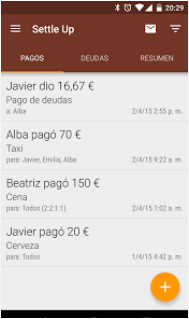
\includegraphics[scale=0.90]{Figures/settleUp1.jpg}
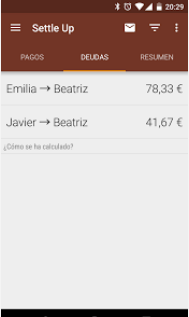
\includegraphics[scale=0.90]{Figures/settleUp2.jpg}
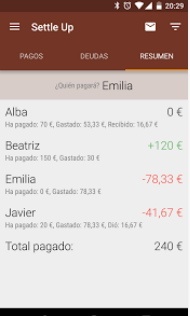
\includegraphics[scale=0.90]{Figures/settleUp3.jpg}
\caption{Settle up}
\end{figure}

\item{\textbf{Splitewise}}\\
Splitewise, aplicació mòbil de control de despeses, ofereix gestió d’usuaris, possibilitat de crear una xarxa d’amics i gestió de divises. En aquesta aplicació també s’hi pot afegir una foto i una categoria a la despesa.

\begin{figure}[!h]
\centering
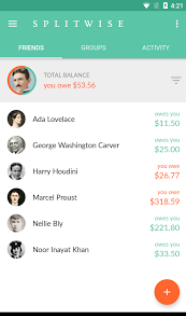
\includegraphics[scale=0.90]{Figures/splitwise1.jpg}
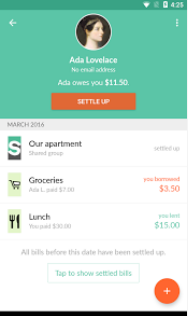
\includegraphics[scale=0.90]{Figures/splitwise2.jpg}
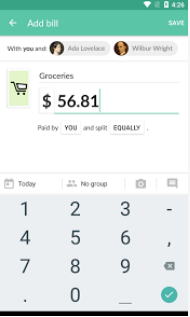
\includegraphics[scale=0.90]{Figures/splitwise3.jpg}
\caption{Splitwise}
\end{figure}

\end{itemize}
\item{\textbf{Previsió metereològica}}\\
En aquest punt s’analitzen les aplicacions de previsió metereològica. Existeixen varies aplicacions molt complertes que controlen la metereologia. Cap d’aquestes, però, està enfocada cap al món viatger, la idea de l’aplicació proposada és mostrar la informació que un viatger necessita saber per decidir què fer durant la seva jornada.\\
S’han analitzat dues aplicacions:
\begin{itemize}
\item{\textbf{Rain Alarm}}\\
Rain Alarm destaca pel seu mapa amb representació gràfica de la probabilitat de pluja a l’instant. També localitza automàticament el punt on es troba l’usuari, avisa en cas de pluja imminent i ofereix l’opció d’ajustar la precisió d’aquest avís. Un dels punts negatius de l’aplicació és que conté publicitat.

\clearpage

\begin{figure}[!h]
\centering
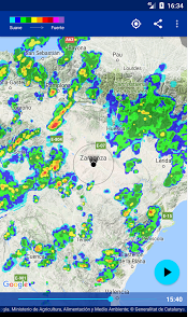
\includegraphics[scale=0.90]{Figures/rainAlarm.jpg}
\caption{Meteoplaza}
\end{figure}

\item{\textbf{Alarma lluvia meteoplaza}}\\
Aquesta aplicació és més simple que l’anterior. Destaca per la representació gràfica de la probabilitat de pluja a l’instant, la localització automàtica i l’avís a l’usuari en cas de pluja imminent.

\begin{figure}[!h]
\centering
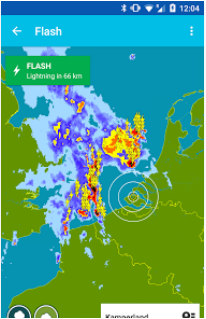
\includegraphics[scale=0.90]{Figures/meteoplaza1.jpg}
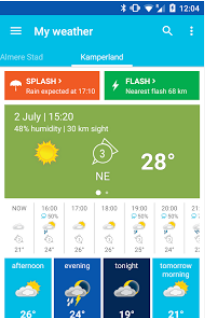
\includegraphics[scale=0.90]{Figures/meteoplaza2.jpg}
\caption{Meteoplaza}
\end{figure}

\end{itemize}
\item{\textbf{Gestió d’emergències}}\\
En aquest punt s’analitzen les aplicacions que tracten el suport en cas d’emergència. L’aplicació que vol crear aquest projecte proposa una funcionalitat que gestioni emergències amb funcionalitats útils per al viatger durant el dia a dia del seu viatge.\\
S’han analitzat dues aplicacions:
\begin{itemize}
\item{\textbf{Emergency Assistant}}\\
Emergency Assistant guarda un perfil personal de l’usuari i emmagatzema contactes a qui acudir en cas d’emergència. Aquestes funcionalitats són les que més s’apropen al que proposa el projecte. A més, també ofereix control d’al·lèrgies, informació sobre l’assegurança, un llistat de medicacions que l’usuari pren i l’historial mèdic. Es considera, però, que aquestes darreres funcionalitats no són prou importants en el context sobre el que es treballa.

\begin{figure}[!h]
\centering
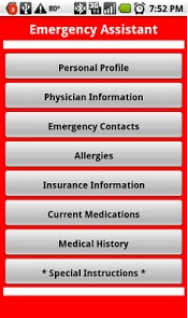
\includegraphics[scale=0.90]{Figures/emerAssistant1.jpg}
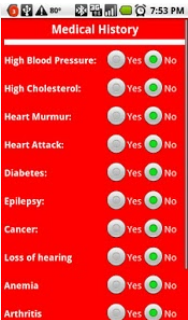
\includegraphics[scale=0.90]{Figures/emerAssistant2.jpg}
\caption{Emergency assistant}
\end{figure}

\item{\textbf{First Call}}\\
First Call ofereix funcionalitats molt interessants pel que fa al punt de vista viatger que té el projecte. Aquesta aplicació és molt més senzilla i es centra en classificar el tipus d’emergència del que es tracta i facilitar molt l’avís a terceres persones en cas d’accident, en aquest cas s’envia un avís a d’altres usuaris de l’aplicació. A més també ofereix informació sobre els telèfons de contacte en cas d’emergència de diferents països.

\begin{figure}[!h]
\centering
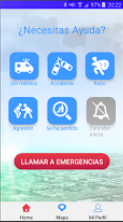
\includegraphics[scale=1.10]{Figures/firstCall1.jpg}
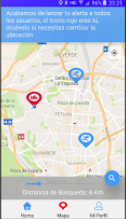
\includegraphics[scale=1.10]{Figures/firstCall2.jpg}
\caption{First Call}
\end{figure}

\end{itemize}
\item{\textbf{Gestió de cerques}}\\
En aquest punt s’analitzen les aplicacions que tenen a veure amb cercar llocs d’interès en un lloc concret.
S’han analitzat les dues aplicacions més utilitzades al moment.
\begin{itemize}
\item{\textbf{Arround me}}\\
Arround me ofereix cerques d’establiments que poden interessar a una persona quan està fora de casa, aquests establiments els ofereix de manera ordenada per categories diferenciant cerca d’hotels, restaurants, gasolineres, etc. A més, també ofereix servei de previsió metereològica.

\begin{figure}[!h]
\centering
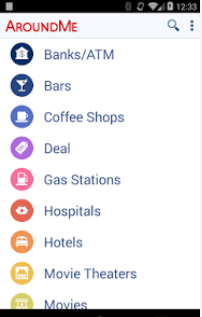
\includegraphics[scale=0.90]{Figures/arroundMe1.jpg}
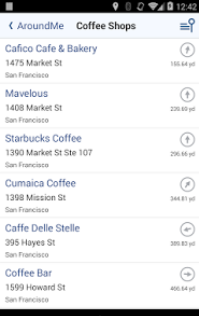
\includegraphics[scale=0.90]{Figures/arroundMe2.jpg}
\caption{Arround me}
\end{figure}

\item{\textbf{Google Maps}}\\
Google Maps és una aplicació molt complerta que ofereix cerques d’establiments, rutes entre un punt i un altre i representació en forma de mapa de tot el món.
D’altra banda, cal dir que cap de les dues aplicacions ofereix una cerca personalitzada per a l’usuari i tampoc està exclusivament enfocat al món viatger. Aquests dos punts són trets distintius d’aquest projecte.

\clearpage

\begin{figure}[!h]
\centering
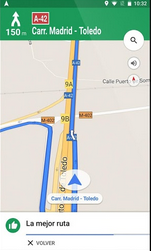
\includegraphics[scale=1.10]{Figures/maps1.jpg}
\caption{Google Maps}
\end{figure}

\end{itemize}
\item{\textbf{Gestió de notes}}\\
En aquest punt s’analitzen les aplicacions que treballen en el camp de les notes escrites. Aquesta funcionalitat no té gairebé res a veure amb el món dels viatges, tot i així es decideix implementar-la ja que es troba interessant oferir un lloc on enregistrar fets curiosos, anècdotes o diferents notes.\\
Existeixen moltes aplicacions que presenten solució a aquest problema, s’han analitzat dues que es considera que es poden apropar a la funcionalitat desitjada.
\begin{itemize}
\item{\textbf{Notes}}\\
Notes és una aplicació gratuïta que ofereix creació de notes amb l’opció d’organitzar-les en carpetes, llistes de verificació i establir recordatoris a la nota. A més, les notes es guarden automàticament quan són creades o modificades. 

\clearpage

\begin{figure}[!h]
\centering
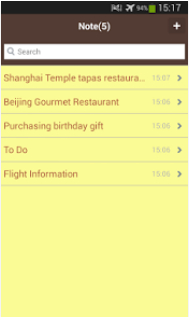
\includegraphics[scale=1.00]{Figures/notes1.jpg}
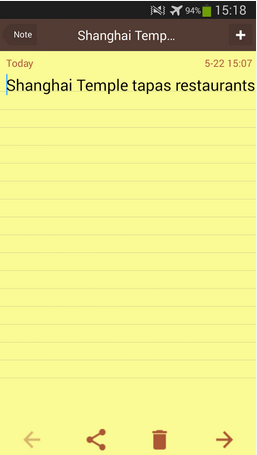
\includegraphics[scale=0.70]{Figures/notes2.jpg}
\caption{Notes}
\end{figure}

\item{\textbf{ColorNote}}\\
ColorNote és una aplicació simple de llibreta que ofereix organització de notes per color, llistes de verificació i possibilitat de posar contrassenya a les notes. L’aplicació, a més, també té recordatori i la possibilitat de compartir notes a través de SMS i correu electrònic.
L’aplicació que proposa aquest projecte pretén oferir un servei bàsic de notes basat en el que pot necessitar el viatger durant el seu viatge. És per aquest motiu que es vol que cada nota estigui localitzada geogràficament i es pugui etiquetar els viatgers.


\begin{figure}[!h]
\centering
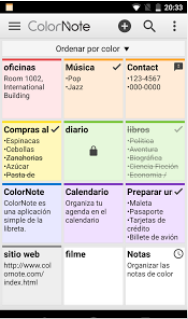
\includegraphics[scale=0.90]{Figures/colorNote1.jpg}
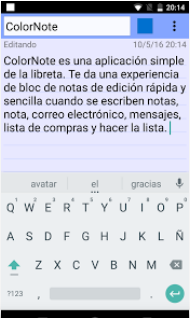
\includegraphics[scale=0.90]{Figures/colorNote2.jpg}
\caption{Color note}
\end{figure}

\end{itemize}
\end{itemize}
\section{Conclusions}
Després d'un anàlisi exhaustiu de la situació actual del mercat pel que fa a aplicacions mòbil que puguin competir amb la idea d'aquest projecte és conclou que realment hi ha un buit en aquest camp.\\

Existeixen, com s'ha exposat en l'apartat anterior, moltes aplicacions que afronten funcionalitats que poden ajudar al viatger durant el trascurs del seu viatge. No obstant, cap d'aquestes aplicacions engloba funcionalitats de vàries temàtiques ni té el món viatger com a temàtica.\\

L'estudi del mercat, ha estat molt útil també, a l'hora de refinar les idees que es tenien sobre que oferir a l'usuari en cada funcionalitat.
